\documentclass{article}
\usepackage[utf8]{inputenc}
\usepackage{graphicx}
\usepackage{enumitem}
\begin{document}
\section{Uvod}
\subsection{"Najmanji problem"}
\subsection{Moguća unapredjenja}
\subsection{Metodologija rada}
\subsection{Korišćeni alati}
\section{Slučajevi upotrebe}
\subsection{Upravljanje ljudskim resursima}
Upravljanje ljudskim resursima je slučaj upotrebe u kojem se definišu rasporedi smena i godišnjih odmora. U planiranju učestvuju radnik i (hr)menadžer.

\begin{itemize}
\item Radnik svoje želje za godišnjim odmorom predaje na odobravanje menadžeru koji te želje skuplja, obradjuje, planira i na kraju daje pozitivan ili negativan odgovor.
\item Raspored smena pravi menažer, koji su potom dostupni na pregled radnicima.
\end{itemize}
%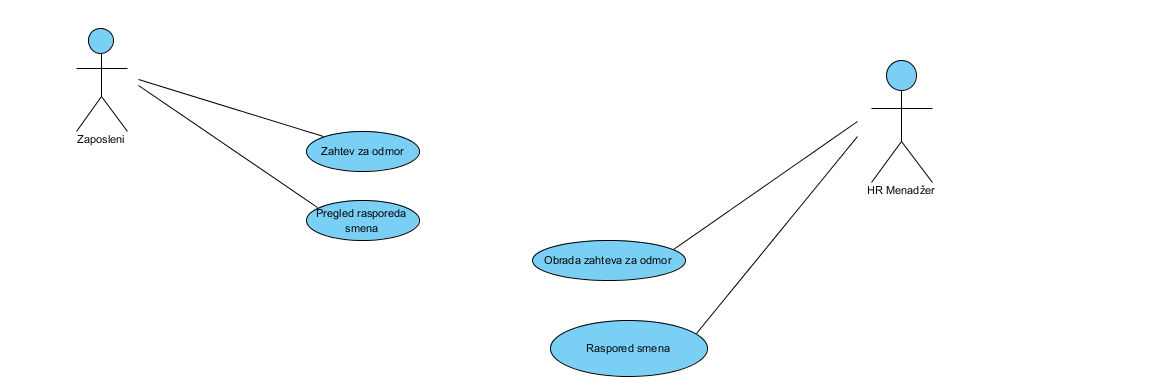
\includegraphics[width=\textwidth]{hr.png}
\subsubsection{\textbf{Use Case}: Zahtev za odmor}
\textbf{Akter:} Radnik\\
\textbf{Ulaz:} Nema\\
\textbf{Izlaz:} Definisan zahtev za odmor\\
\textbf{Preduslovi:} Radnik poseduje username i lozinku za prijavljivanje na glavni sistem gde se definišu zahtevi\\
\textbf{Postuslov:} Uspešno poslat zahtev za odmor\\
\textbf{Glavni tok:} Radnik na osnovu svojih potreba i želja šalje zahtev za godišnji odmor putem glavnog sistema, gde definiše početak i kraj odmora.\\
\textbf{Alternativni tok:} Prijavljivanje nije uspešno, zahtev se ne može napraviti\\

\subsubsection{\textbf{Use Case}: Obrada zahteva za odmor}
\textbf{Akter:} Menadžer\\
\textbf{Ulaz:} Spiskovi zahteva za odmor\\
\textbf{Izlaz:} Definisani odgovori na zahteve\\
\textbf{Preduslovi:}Menadžer se uspešno ulogovao na sistem i spiskovi zahteva su uspešno stigli do njega\\
\textbf{Postuslov:} Odgovori su definisani\\
\textbf{Glavni tok:} Menadžer uzima spiskove zahteva za odmor i procenjuje ukoliko radnici imaju dovoljan broj preostalih slobodnih dana, da li je moguće organizovati funkcionisanje restorana u datom periodu bez dotičnog radnika, da li je zakonom definisano da radnik mora uzeti odmor(npr. ukolko mu je ostao odmor od prethodne godine). Na osnovu procene stanja donosi se odluka.
\textbf{Alternativni tok:} Ukoliko su navedeni zahtevi za slobodnim danima definisani zakonom(slava, selidba, smrtni slučaj, rodjenje deteta,..) dani se odobravaju bez dodatnih procena\\
\subsubsection{\textbf{Use Case}: Raspored smena}
\textbf{Akter:} Menadžer\\
\textbf{Ulaz:} Nema\\
\textbf{Izlaz:} Novi raspored smena za odredjeni period\\
\textbf{Preduslovi:} Postoje informacije o planu rada restorana za dati period kao i spisak godišnjih odmora\\
\textbf{Postuslov:}Sastavjen je novi raspored smena za odredjeni period i spreman je za slanje\\
\textbf{Glavni tok:} Menadžer definiše rasporede smena, za odredjeni period, na osnovu plana rada restorana i definisanih godišnjih odmora\\
\textbf{Alternativni tok:} Zbog promene plana rada restorana ili odsustva radnika, već postojeći raspored mora da se menja\\

\subsubsection{\textbf{Use Case}: Pregled rasporeda smena}
\textbf{Akter:} Radnik\\
\textbf{Ulaz:} Nema\\
\textbf{Izlaz:} Raspored smena za radnika\\
\textbf{Preduslovi:} Radnik poseduje username i lozinku za prijavljivanje na glavni sistem\\
\textbf{Postuslov:} Uspešan pregled smena\\
\textbf{Glavni tok:}Radnik može da vidi svoj raspored smena i u skladu sa tim da dolazi na posao\\
\textbf{Alternativni tok:}Još nije definian raspored smena za željeni period, radnik nema šta da vidi\\
%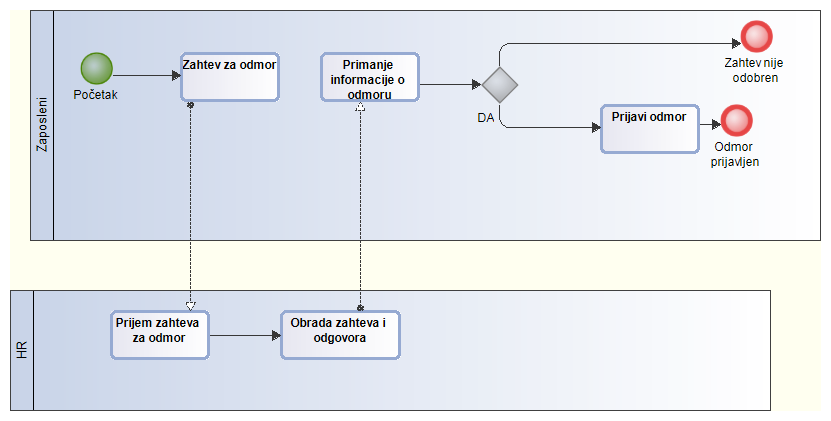
\includegraphics[width=\textwidth]{Odmor.png}\\
%\includegraphics[width=\textwidth]{Raspored_smena.png}\\
\section{Baza podataka}
\section{Predlog korisničkog interfejsa}
\section{Prototip}
\end{document}
